\section{Position du problème}
Nous avons décider de séparer notre logiciel en 2 tâches temps réel : \begin{itemize}
\item \emph{void generateur} : fonction de haute priorité qui s'occupe de générer les 2 signaux sinusoïdaux. 
\item \emph{void lecture} : fonction qui va lire les valeurs en entrées (potentiomètre et numérique) pour recalculer les signaux.
\end{itemize}
Au vue de ces deux tâches, il est impératif de décider maintenant de la différence de priorité entre ces deux taches principale. Il nous semble approprier, à ce stade de l'implémentation, de donner plus de priorité à la fonction \emph{void generateur} pour permettre un rafraichissement de la valeur envoyé sur le convertisseur numérique analogique suffisante. La fonction \emph{void lecture} sera alors appelée moins régulièrement que la génération des signaux.
\subsection{Génération du signal périodique}
\label{subsection:signalperiodique}
Les calculs dans un programme temps réel ne sont généralement pas souhaitables : il demande trop de temps, selon leur complexité, au processeur. Selon cette affirmation, pour générer les signaux sinusoïdaux, nous ne devons faire aucun calcul de $\sin$ dans le programme principal. Nous devons générer d'une autre manière un série de 50 valeurs comprises entre [-1;1] qui représente notre signal sinusoïdal qui n'a pas subit de modifications.

\begin{center}
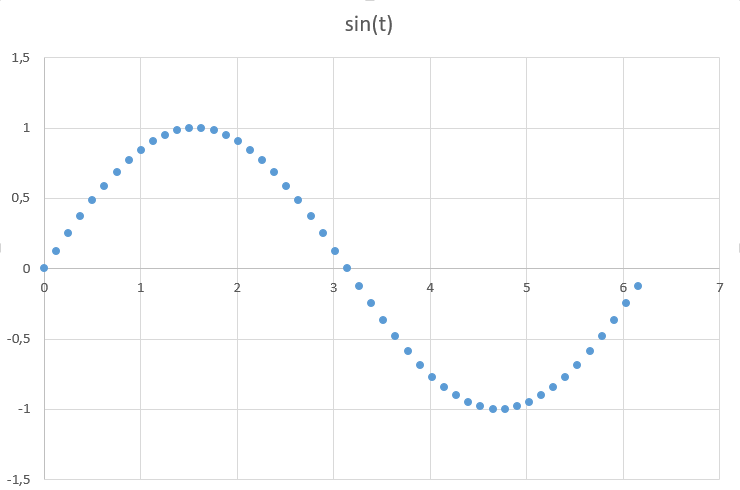
\includegraphics[width = .7\textwidth]{./II/images/sinus.png}
\captionof{figure}{Signal sinusoïdal enregistré dans le tableau}
\end{center}
\subsection{Conversion des valeurs analogique vers numérique}
Pour pouvoir sortir un signal analogique, le programme RTAI utilise un convertisseur numérique-analogique 16 bits avec la librairie \emph{comedio}. Il nous faut adapter les valeurs en V que nous souhaitons envoyer à ces valeurs numériques. Nous allons utiliser la loi suivante qui a été calculé en sachant que le signal peut avoir une amplitude max de [-10V; 10V]. Avec ces informations, nous trouvons : \begin{align*}
S_{data} = \frac{65535}{20}\times V + 32767
\end{align*}

\subsection{Envoie des signaux sur le CNA}
L'implémentation de la tâche de haute priorité nécessite de commencer par l'initialisation RTAI de celle-ci. Nous décidons de mettre une fréquence fixe pour commencer de 1ms  
\begin{lstlisting}[style = customc]
int init_module(void)
{	 
 // Initialisation de la carte d'E/S
  cf = comedi_open("/dev/comedi0");	
  if(cf == NULL)
  {
    comedi_perror("Comedi fails to open");
    return -1;
  }

   	// OUTPUTS

	rt_set_oneshot_mode();
	// Lancement du timer

	now =  start_rt_timer(0); // creation timer de periode  50ms
 	now = rt_get_time();
  	// Lancement des taches
  		// lecture 
	 
			
  		// generateur  
 	rt_task_init( &generateur_ptr, 	/* Le prt de tache */
	 	      generateur1,	   	/* Nom de la tache */
	 	      1, 		/* valeur du parametre X */
	 	      2000,		/* Taille de la pile necessaire pour la tache (memoire tempo utilisee) */
	 	      0,		/* Priorite */
	 	      1,  		/* Calcul flottant */
	 	      0); 		/* choix d'un signal ou non  */
	 	      

	rt_task_make_periodic(	&generateur_ptr, 	/* Pointeur vers la tache */
				now,		/* Instant de depart */
				nano2count(s1_period*ms/SIZETAB));		/* Periode */

  return 0;
}
\end{lstlisting}
La tâche de génération de signaux consiste à exécuter dans une boucle infinie la lecture de la case du tableau des valeurs possibles du sinus, convertir cette valeur pour le CNA de 16bits et l'envoyer avec \emph{comedi\_data\_write}. Cette boucle attend ensuite sa prochaine ré-activation pour recommencer ces opérations en décalant sa lecture des données générés dans \ref{subsection:signalperiodique}.
\begin{lstlisting}[style = customc]
void generateur1 (long int x)
{
	unsigned int 	data; //[0 ;2^32 -1]

	while (1)//loop
	{  
	  	data = (unsigned int)(32767.5 + 65535/20*(s1_alpha*signal_sin[s1_i])); // A*sin(2pif)
	  	comedi_data_write(cf, CNA, CHAN_0, RANGE, AREF, data);
	  	s1_i = (s1_i+1)%SIZETAB;								// Passer toute les cases du tableau
	  	rt_task_wait_period();									// Jusqu'a la prochaine periode
	}
}
\end{lstlisting}

\subsection{Observation des résultats}
Nous observons deux signaux échantillonnés sur l'écran de notre oscilloscope qui sont similaires. Il semble que l'implémentation du reste de l'application soit possible. 